\chapter{ठोसों में इलेक्ट्रॉन}\label{ch:b3:electrons-in-solids}

% Provenance (not for print): second half of the "physique du solide"
% module (Drude, Sommerfeld, bands, semiconductors) common to the
% surveyed third-year curricula.

ताँबा क्वार्ट्ज़ से दस लाख अरब अरब गुना बेहतर बिजली चलाता है --- किसी
भी भौतिक गुण का सबसे चौड़ा परास, और वह भी ऐसे पदार्थों के हाथ में जो
दोनों हालत में भूरे ढेलों जैसे दिखते हैं। पिछले अध्याय का ढाँचा इसमें
से कुछ नहीं समझाता; और उसमें उँडेले गए \emph{इलेक्ट्रॉन} सब कुछ समझा
देते हैं। यह अध्याय इस समस्या पर सदी के तीन प्रहार चलाता है, जिनमें
हर एक पिछले का मलबा विरासत में पाता है: ड्रुडे की चिरसम्मत पिनबॉल
(1900), जो ओम का नियम सही पाती है और ऊष्माधारिता शर्मनाक ढंग से ग़लत;
ज़ोमरफ़ेल्ट की फ़र्मी गैस, जो \cref{ch:b3:quantum-statistics} के चेक को
भुनाना भर है; और ब्लॉख की सूझ कि किसी आवर्ती \omterm{def:b3:crystalline-solids:lattice}{जालक} में
इलेक्ट्रॉन-तरंग हर दूसरी तरंग की तरह ब्रैग-परावर्तित होती है --- और
इससे \emph{\omterm{thm:b3:electrons-in-solids:bloch}{बैंड अंतराल}} खुलते हैं, जो सारे ठोसों को धातुओं,
विद्युत्रोधियों, और सँकरे-अंतराल वाली उन मँझली संतानों,
अर्धचालकों, में छाँट देते हैं, जिन पर पूरा इलेक्ट्रॉनिक युग खड़ा है।
अध्याय किसी सौर पैनल के भीतर जाकर समाप्त होता है।

\section{ड्रुडे की पिनबॉल धातु}

\begin{proposition}[ड्रुडे चालकता]\label{prop:b3:electrons-in-solids:drude}
\index{ड्रुडे प्रतिरूप}\index{चालकता!सूक्ष्म}\index{अपवाह वेग}
किसी \omterm{def:b3:electrons-in-solids:classes}{धातु} के संयोजी इलेक्ट्रॉनों को घनत्व $n$ की कोई चिरसम्मत गैस
मानिए, जो हर $\tau$ सेकंड पर बाधाओं से टकराती हो। कोई क्षेत्र $\vect E$
हर एक को संघट्टों के बीच त्वरित करता है; और औसत \emph{\omterm{prop:b3:electrons-in-solids:drude}{अपवाह
वेग}} $\vect v_{\text{d}} = -e\tau\vect E/m_{\text{e}}$ है,
जो तापीय गति के आगे नन्हा है। तब धारा घनत्व $\vect j =
-ne\vect v_{\text{d}}$ स्थानीय रूप से ओम का नियम मानता है,
$\vect j = \sigma\vect E$, जहाँ
\[
\sigma = \frac{ne^2\tau}{m_{\text{e}}} .
\]
ताँबे का मापा गया $\sigma$ $\tau \approx \qty{2.5e-14}{s}$ माँगता है
--- और इस प्रतिरूप के दो गौरव इसी से निकलते हैं: यह समझाता है कि
प्रतिरोधक गरम क्यों होते हैं (क्षेत्र का कार्य हर संघट्ट पर तापीय हो
जाता है), और यह वीडेमान--फ़्रांत्स नियम की भविष्यवाणी करता है कि
$\kappa/\sigma T$ सारी धातुओं के लिए वही नियतांक है --- क्योंकि
इलेक्ट्रॉन आवेश और ऊष्मा, दोनों ढोते हैं
(\cref{exo:b3:electrons-in-solids:5})।
\end{proposition}

\begin{proof}
संघट्टों के बीच $\dot{\vect v} = -e\vect E/m_{\text{e}}$;
और हर संघट्ट पर नए सिरे से शुरू करने पर किसी माध्य काल
$\tau$ में अर्जित माध्य वेग $-e\tau\vect E/m_{\text{e}}$ है। तब $\vect j =
-ne\vect v_{\text{d}} = (ne^2\tau/m_{\text{e}})\vect E$।
\end{proof}

\begin{omfigure}
\begin{tikzpicture}[scale=1.0]
  % ion grid
  \foreach \x in {0,1.3,...,7.9}
    \foreach \y in {0,1.1,2.2}
      \draw[omDef!50, fill=omDef!12] (\x,\y) circle (5.5pt);
  % zigzag electron path with slight downfield drift
  \draw[omThm, thick, ->]
    (0.25,1.62) -- (1.0,0.55) -- (1.9,1.7) -- (2.6,0.6) -- (3.6,1.55)
    -- (4.3,0.45) -- (5.25,1.6) -- (5.95,0.5) -- (6.9,1.5) -- (7.65,0.7);
  % field and drift arrows
  \draw[->, thick] (2.6,3.0) -- (1.2,3.0)
    node[midway, above, font=\scriptsize] {$\vect E$};
  \draw[->, thick, omThm, dashed] (5.0,3.0) -- (6.8,3.0)
    node[midway, above, font=\scriptsize]
    {अपवाह $\vect v_{\text{d}}$};
\end{tikzpicture}

{\small ड्रुडे का चित्र: कोई इलेक्ट्रॉन
$\sim\qty{e6}{m/s}$ पर उछलता-टकराता है, जबकि क्षेत्र उस पर प्रति
सेकंड मिलीमीटर के अंशों जितना अपवाह चढ़ा देता है
(\cref{exo:b3:electrons-in-solids:2})। ओम का नियम अपने आप निकल आता
है; और इस प्रतिरूप की विफलताओं ने उससे भी अधिक सिखाया।}
\end{omfigure}

\begin{remark}[ज़ोमरफ़ेल्ट का बचाव]\label{rem:b3:electrons-in-solids:sommerfeld}
\index{ज़ोमरफ़ेल्ट प्रतिरूप}\index{फ़र्मी ऊर्जा!धातुओं में}
ड्रुडे की गैस को किसी \omterm{def:b3:electrons-in-solids:classes}{धातु} की ऊष्माधारिता में प्रति इलेक्ट्रॉन
$\tfrac32k_{\text{B}}$ जोड़ना चाहिए; पर प्रयोग सौ गुना कम पाता है।
\Cref{ch:b3:quantum-statistics} इलेक्ट्रॉनों को पहले ही बरी कर चुका
है: वे एक \emph{अपह्रासित फ़र्मी गैस} हैं, $T_{\text{F}} \sim
\qty{8e4}{K}$, और केवल फ़र्मी सतह के
$k_{\text{B}}T$ भीतर वाला तापीय कोश ही अनुक्रिया कर सकता है --- ऊष्मा
पर भी, और प्रकीर्णन पर भी। ज़ोमरफ़ेल्ट ने ड्रुडे को फ़र्मी--डिराक
सांख्यिकी के साथ फिर से चलाया, जिसमें चालकता का सूत्र बना रहता है (और
$\tau$ अब फ़र्मी-सतह के इलेक्ट्रॉनों का जीवनकाल है, जिनकी
\qty{e6}{m/s} तापीय चाल नहीं बल्कि
$v_{\text{F}}$ है), ऊष्माधारिता सुधरकर अपने मापे गए
$T/T_{\text{F}}$ वाले पतले टुकड़े पर आ जाती है, और
वीडेमान--फ़्रांत्स का संख्यात्मक नियतांक तक ठीक हो जाता है। पर हर
मुक्त-इलेक्ट्रॉन प्रतिरूप के बाद भी एक रहस्य बचा रहता है: क्वार्ट्ज़
बिलकुल भी चालन क्यों नहीं करता।
\end{remark}

\section{ब्लॉख: जालक बोलता है}

\begin{theorem}[ब्लॉख अवस्थाएँ और बैंड अंतराल]\label{thm:b3:electrons-in-solids:bloch}
\index{ब्लॉख की प्रमेय}\index{बैंड अंतराल}\index{बैंड संरचना}
किसी निर्दोष आवर्ती विभव में अचर अवस्थाएँ
\emph{ब्लॉख तरंगें} $\psi_k(x) = u_k(x)\eu^{\iu kx}$ हैं ---
यानी \omterm{def:b3:crystalline-solids:lattice}{जालक} की अपनी आवर्तिता $u_k$ से सजी समतल तरंगें ---
जो \emph{बिना प्रकीर्ण हुए} संचरित होती हैं: किसी निर्दोष \omterm{def:b3:crystalline-solids:lattice}{क्रिस्टल} का
प्रतिरोध शून्य होता है, और असली प्रतिरोध खामियों से आता है
(कंपन, अशुद्धियाँ)। पर हर ऊर्जा बचती नहीं। $k = \pi/a$ पर
इलेक्ट्रॉन की तरंगदैर्घ्य $2a$ होती है: यानी स्वयं \omterm{def:b3:crystalline-solids:lattice}{जालक} पर ब्रैग की
शर्त (\cref{thm:b3:crystalline-solids:dispersion} ने ध्वनि के लिए
यही खोज की थी)। परावर्तित और आपाती तरंगें दो अप्रगामी प्रतिरूप बनाती
हैं --- आवेश आयनों पर ढेर (कम ऊर्जा) या उनके बीच (अधिक) --- अतः
मुक्त-इलेक्ट्रॉन परवलय $E = \hbar^2k^2/2m_{\text{e}}$ चिर जाता है:
वर्जित ऊर्जाओं का एक अंतराल, यानी \emph{\omterm{thm:b3:electrons-in-solids:bloch}{बैंड अंतराल}} $E_{\text{g}}$,
अनुमत अवस्थाओं के एक भरे-पूरे \emph{बैंड} को अगले से अलग कर देता है।
किसी \omterm{def:b3:crystalline-solids:lattice}{क्रिस्टल} की इलेक्ट्रॉनी पहचान उसकी बैंडों और अंतरालों की सीढ़ी है।
\end{theorem}
\admitted

\begin{omfigure}
\begin{tikzpicture}
  \begin{axis}[omaxis, axis x line=bottom, axis y line=left,
    width=9.6cm, height=6.2cm, xmin=0, xmax=5.4, ymin=0, ymax=2.6,
    xlabel={$k$}, ylabel={$E$},
    xlabel style={at={(axis description cs:0.5,-0.1)}, anchor=north},
    xtick={3.1416}, xticklabels={$\pi/a$}, ytick=\empty, clip=true]
    % free-electron parabola (dashed)
    \addplot[gray, dashed, domain=0:5.1, samples=120] {x*x/10};
    % lower band: bends flat at zone edge
    \addplot[omDef, very thick, domain=0:3.1416, samples=120]
      {x*x/10 - 0.18*(x/3.1416)^6};
    % upper band
    \addplot[omDef, very thick, domain=3.1416:5.1, samples=120]
      {x*x/10 + 0.18*((5.1-x)/1.9584)^2};
    \draw[gray, dashed] (axis cs:3.1416,0) -- (axis cs:3.1416,2.55);
    % gap markers
    \draw[omThm, thick, <->] (axis cs:3.2,0.81) -- (axis cs:3.2,1.16);
    \node[omThm, font=\scriptsize, anchor=west] at (axis cs:3.34,0.98)
      {अंतराल $E_{\text{g}}$};
    \node[gray, font=\scriptsize, anchor=north west, align=left]
      at (axis cs:0.35,2.45) {बिंदुदार: मुक्त इलेक्ट्रॉन};
    \node[omDef, font=\scriptsize, anchor=east] at (axis cs:2.75,0.35)
      {बैंड 1};
    \node[omDef, font=\scriptsize, anchor=west] at (axis cs:3.6,2.35)
      {बैंड 2};
  \end{axis}
\end{tikzpicture}

{\small लगभग-मुक्त इलेक्ट्रॉन। क्षेत्र-किनारे से दूर वह
इलेक्ट्रॉन \omterm{def:b3:crystalline-solids:lattice}{जालक} को मुश्किल से भाँपता है; और $k = \pi/a$ पर उसका अपना
ब्रैग परावर्तन उस परवलय को चीर देता है, जिससे अंतराल की ऊर्जाएँ वर्जित
हो जाती हैं। पिछले अध्याय में ध्वनि-तरंगों ने ठीक यही किया था --- वही
\omterm{def:b3:crystalline-solids:lattice}{जालक}, वही व्यतिकरण, नया किरायेदार।}
\end{omfigure}

\begin{definition}[धातु, विद्युत्रोधी, अर्धचालक]\label{def:b3:electrons-in-solids:classes}
\index{धातु}\index{विद्युत्रोधी}\index{अर्धचालक}
बैंडों को \omterm{def:b3:crystalline-solids:lattice}{क्रिस्टल} के इलेक्ट्रॉनों से भरिए, प्रति अवस्था दो
(\cref{ch:b3:identical-particles}), और पहले सबसे ठंडी। यदि सबसे ऊपर
की अधिभुक्त बैंड \emph{आंशिक} रूप से भरी हो, तो अत्यल्प ऊर्जा भी
इलेक्ट्रॉनों को शुद्ध गति में खिसका सकती है: वह एक \emph{धातु} है
(सोडियम: एक संयोजी इलेक्ट्रॉन, आधी बैंड; और द्विसंयोजी धातुएँ
अतिव्यापी बैंडों से चालन करती हैं)। यदि वह \emph{ठीक-ठीक} भरी हो और
ऊपर कोई चौड़ा अंतराल हो, तो कोई छोटा धक्का कुछ भी पुनर्व्यवस्थित नहीं
कर सकता: वह एक \emph{विद्युत्रोधी} है
(हीरा, $E_{\text{g}} = \qty{5.5}{eV}$)। और यदि वह अंतराल छोटा हो ---
सिलिकॉन में $\qty{1.12}{eV}$ --- तो तापीय हलचल कुछ इलेक्ट्रॉनों को
पार चढ़ा देती है, और हर एक नीचे एक गतिशील \emph{\omterm{def:b3:electrons-in-solids:doping}{विवर}} छोड़ जाता है: वह
एक \emph{अर्धचालक} है, जिसकी वाहक-संख्या
$\propto\eu^{-E_{\text{g}}/2k_{\text{B}}T}$ कुछ ही अंशों में दुगनी हो
जाती है। इसी से वह महान विभाजन: धातुएँ गरम करने पर बदतर चालन करती हैं
(प्रकीर्ण करने को अधिक कंपन), और अर्धचालक बेहतर
(चरघातांकी रूप से अधिक वाहक) --- एक ही चिह्न-पलटाव, जो किसी पदार्थ का
वर्ग एक ही मापन में पहचान देता है।
\end{definition}

\begin{omfigure}
\begin{tikzpicture}[scale=1.0]
  % metal: half-filled band
  \begin{scope}
    \fill[omDef!25] (0,0) rectangle (1.8,0.8);
    \draw[thick] (0,0) rectangle (1.8,1.6);
    \node[font=\scriptsize, anchor=north] at (0.9,-0.15) {धातु};
    \node[font=\tiny, anchor=south] at (0.9,1.65) {आंशिक भरी};
  \end{scope}
  % insulator
  \begin{scope}[xshift=3.6cm]
    \fill[omDef!25] (0,0) rectangle (1.8,0.9);
    \draw[thick] (0,0) rectangle (1.8,0.9);
    \draw[thick] (0,2.1) rectangle (1.8,2.9);
    \draw[omThm, thick, <->] (2.05,0.9) -- (2.05,2.1);
    \node[omThm, font=\tiny, anchor=west] at (2.12,1.5)
      {$E_{\text{g}} \sim \qty{5}{eV}$};
    \node[font=\scriptsize, anchor=north] at (0.9,-0.15) {विद्युत्रोधी};
    \node[font=\tiny, anchor=south] at (0.9,2.95) {खाली};
  \end{scope}
  % semiconductor
  \begin{scope}[xshift=8.4cm]
    \fill[omDef!25] (0,0) rectangle (1.8,0.9);
    \draw[thick] (0,0) rectangle (1.8,0.9);
    \draw[thick] (0,1.5) rectangle (1.8,2.3);
    \draw[omThm, thick, <->] (2.05,0.9) -- (2.05,1.5);
    \node[omThm, font=\tiny, anchor=west] at (2.12,1.2)
      {$\sim\qty{1}{eV}$};
    % thermally excited carriers
    \fill[omThm] (0.5,1.62) circle (1.6pt);
    \fill[omThm] (1.25,1.62) circle (1.6pt);
    \draw[omThm] (0.5,0.78) circle (1.6pt);
    \draw[omThm] (1.25,0.78) circle (1.6pt);
    \node[font=\scriptsize, anchor=north] at (0.9,-0.15) {अर्धचालक};
    \node[font=\tiny, anchor=south] at (0.9,2.35)
      {कुछ इलेक्ट्रॉन $+$ विवर};
  \end{scope}
\end{tikzpicture}

{\small बैंड का भराव ही सब कुछ तय करता है। कोई आंशिक भरी बैंड
चालन करती है; किसी चौड़े अंतराल के नीचे कोई भरी बैंड नहीं कर सकती; और
कोई सँकरा अंतराल ताप (या प्रकाश, या \omterm{def:b3:electrons-in-solids:doping}{अपमिश्रण}) से सौदा करने देता है ---
\omterm{def:b3:electrons-in-solids:classes}{अर्धचालक} की पूरी उपयोगिता यही है कि उसकी चालकता \emph{समायोज्य} है।}
\end{omfigure}

\section{अंतराल गढ़ना: अपमिश्रण और संधि}

\begin{definition}[अपमिश्रण]\label{def:b3:electrons-in-solids:doping}
\index{अपमिश्रण}\index{दाता}\index{ग्राही}\index{विवर}
दस लाख में से एक सिलिकॉन परमाणु की जगह फ़ॉस्फ़ोरस (पाँच संयोजी
इलेक्ट्रॉन) रख दीजिए: चार बंध संतुष्ट हो जाते हैं और पाँचवाँ
इलेक्ट्रॉन, जो मात्र \qty{45}{meV} से बँधा है
(\cref{exo:b3:electrons-in-solids:10}), कमरे के ताप पर मुक्त हो जाता
है। ऐसे \emph{दाता} किसी \emph{n-प्रकार}
\omterm{def:b3:electrons-in-solids:classes}{अर्धचालक} को जन्म देते हैं, जिसमें चालन इलेक्ट्रॉनों से होता है; जबकि
बोरॉन (तीन इलेक्ट्रॉन) एक \emph{ग्राही} है, जो किसी बंध का इलेक्ट्रॉन
झपट लेता है और एक गतिशील \emph{विवर} छोड़ देता है --- यानी कोई अनुपस्थित
इलेक्ट्रॉन, जो चलता है, क्षेत्रों पर अनुक्रिया करता है, और धन आवेश
उतनी ही सच्चाई से ढोता है जितनी सच्चाई से कोई बुलबुला उत्प्लावन:
यही \emph{p-प्रकार} है। अपमिश्रण वाहक-घनत्व --- और इसलिए चालकता ---
को इच्छानुसार छह कोटियों तक झुला देता है: वही घुंडी, जो रेत को
परिपथों में बदल देती है।
\end{definition}

\begin{proposition}[P--N संधि]\label{prop:b3:electrons-in-solids:junction}
\index{P--N संधि}\index{डायोड}\index{अवक्षय क्षेत्र}
p-प्रकार को n-प्रकार से जोड़िए। इलेक्ट्रॉन विवरों की ओर छलक जाते हैं
और अंतरापृष्ठ के पास उन्हें मिटा देते हैं, जिससे स्थिर आयनित
अपमिश्रकों का एक \emph{\omterm{prop:b3:electrons-in-solids:junction}{अवक्षय क्षेत्र}} उघड़ आता है, और उसकी दोहरी परत
भीतर एक क्षेत्र खड़ा कर देती है --- सिलिकॉन में संतुलन अंतर्निर्मित
वोल्टता $V_{\text{bi}} = (k_{\text{B}}T/e)
\ln(N_{\text{a}}N_{\text{d}}/n_{\text{i}}^2) \approx
\qty{0.7}{V}$ पर आता है। तब वह संधि दिष्टकरण करती है: अग्र
अभिनति उस रोधिका को नीचा करती है और धारा
$\eu^{eV/k_{\text{B}}T}$ की तरह बढ़ती है; जबकि उत्क्रम अभिनति उसे ऊँचा
कर देती है और केवल कोई रिसाव $I_0$ बहता है:
\[
I = I_0\big(\eu^{eV/k_{\text{B}}T} - 1\big) .
\]
यही असममिति \emph{डायोड} है --- और अपने रूपांतरों में यही
LED (पुनर्योजित युग्म अंतराल-ऊर्जा के फ़ोटॉन उत्सर्जित करते हैं), यही
सौर सेल (अंतराल-ऊर्जा के फ़ोटॉन युग्म बनाते हैं, जिन्हें अंतर्निर्मित
क्षेत्र बुहार ले जाता है: \cref{pb:b3:electrons-in-solids:1}), और
सैंडविच की तरह दुगुना करने पर यही ट्रांज़िस्टर है: वही स्विच, जिसे
कोई आधुनिक चिप सैकड़ों अरबों की संख्या में छापती है।
\end{proposition}
\admitted

\begin{omfigure}
\begin{tikzpicture}
  \begin{axis}[omaxis,
    width=9.4cm, height=5.8cm, xmin=-4.6, xmax=3.6, ymin=-5, ymax=16,
    axis lines=middle,
    xlabel={$eV/k_{\text{B}}T$}, ylabel={$I/I_0$},
    xlabel style={anchor=north east},
    xtick=\empty, ytick=\empty, clip=true]
    \addplot[omDef, very thick, domain=-4.5:2.83, samples=200]
      {exp(x) - 1};
    \addplot[gray, dashed, domain=-4.6:0] {-1};
    \node[gray, font=\scriptsize, anchor=north] at (axis cs:-2.7,-1.7)
      {उत्क्रम: रिसाव $-I_0$};
    \node[omDef, font=\scriptsize, anchor=east, align=right]
      at (axis cs:2.5,11.5) {अग्र:\\$\eu^{eV/k_{\text{B}}T}$};
  \end{axis}
\end{tikzpicture}

{\small डायोड का नियम। अग्र वोल्टता चरघातांकी ढंग से लौटाई जाती है;
जबकि उत्क्रम वोल्टता केवल रिसाव $I_0$ खरीदती है। एक संधि
दिष्टकरण करती है; दो मिलकर ट्रांज़िस्टर बनाती हैं; और उनका एक वर्ग
मीटर, धूप में, एक बिजलीघर।}
\end{omfigure}

\begin{omfigure}
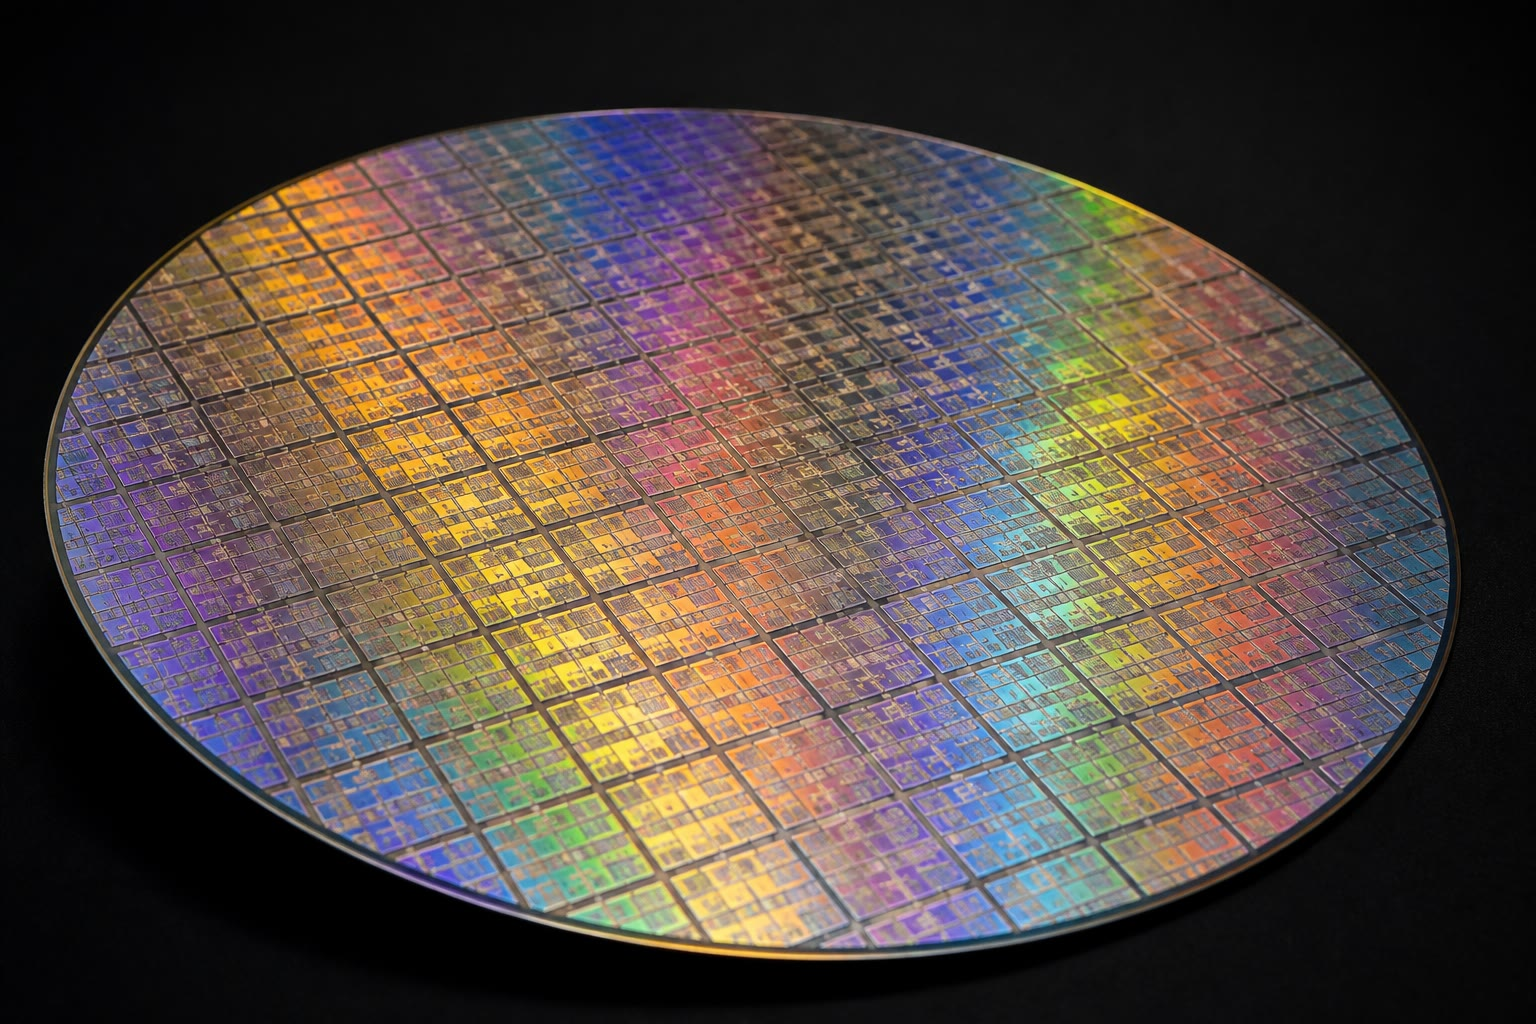
\includegraphics[width=0.58\linewidth]{images/book5/ai/b5-20-silicon-wafer.jpg}

{\small कोई तैयार सिलिकॉन वेफ़र: सैकड़ों चिप, हर एक में अरबों संधियाँ, और सब एक ही अपमिश्रित \omterm{def:b3:crystalline-solids:lattice}{क्रिस्टल} में छपी हुईं --- बैंड सिद्धांत, बीसवीं सदी की सबसे परिणामदायी निर्माण-विधि के रूप में।}
\end{omfigure}

\section{अभ्यास}

\begin{exercise}[$\star$]\label{exo:b3:electrons-in-solids:1}
ड्रुडे का ताँबा। $n = \qty{8.5e28}{m^{-3}}$, प्रतिरोधकता
$\rho = \qty{1.7e-8}{\ohm.m}$। निकालिए: (क) $\tau =
m_{\text{e}}/ne^2\rho$; (ख) फ़र्मी वेग
$v_{\text{F}} = \qty{1.6e6}{m/s}$ से माध्य मुक्त पथ; (ग) वही पथ
\omterm{def:b3:crystalline-solids:lattice}{जालक} नियतांकों में ($a = \qty{3.61}{\angstrom}$); (घ) समझाइए कि
इतनी लंबी उड़ान अभी से क्यों इशारा करती है कि प्रकीर्णन स्वयं आयन नहीं
करते।
\end{exercise}

\begin{exercise}[$\star$]\label{exo:b3:electrons-in-solids:2}
तार में घोंघा। कोई \qty{1}{mm^2} का ताँबे का तार
\qty{10}{A} ढोता है। (क) \omterm{prop:b3:electrons-in-solids:drude}{अपवाह वेग} निकालिए। (ख) किसी
\qty{1}{m} के लैंप-तार को पार करने में किसी इलेक्ट्रॉन को कितना समय
लगेगा? (ग) फिर भी लैंप तुरंत क्यों जल उठता है? (घ)
$v_{\text{d}}$ की $v_{\text{F}}$ से तुलना कीजिए और ड्रुडे के
पिनबॉल चित्र पर टिप्पणी कीजिए।
\end{exercise}

\begin{exercise}[$\star$]\label{exo:b3:electrons-in-solids:3}
बैंडों से छँटाई। बैंड-भराव के नियम से वर्गीकृत कीजिए: (क)
सोडियम (एक संयोजी इलेक्ट्रॉन); (ख) मैग्नीशियम (दो --- फिर भी
\omterm{def:b3:electrons-in-solids:classes}{धातु}: उसकी बैंडों को क्या करना पड़ता है?); (ग) हीरा
($E_{\text{g}} = \qty{5.5}{eV}$); (घ) सिलिकॉन
($\qty{1.12}{eV}$) --- और हर एक के लिए
$\dd\rho/\dd T$ का चिह्न बताइए।
\end{exercise}

\begin{exercise}[$\star$]\label{exo:b3:electrons-in-solids:4}
अंतराल और फ़ोटॉन। (क) कौन-सी फ़ोटॉन तरंगदैर्घ्य सिलिकॉन के अंतराल से
मेल खाती है, और सिलिकॉन किस वर्णक्रमीय क्षेत्र में पारदर्शी हो जाता
है? (ख) हीरे के लिए भी वही: वह दृश्य में साफ़ क्यों है? (ग) गैलियम
नाइट्राइड के किसी LED का $E_{\text{g}} =
\qty{3.4}{eV}$ है: वह कौन-सा रंग-किनारा तय करता है, और नीले
LED को यही पदार्थ क्यों चाहिए था? (घ) कोई लाल LED अधिक चलाने पर
मंद सफ़ेद चमकने के बजाय अँधेरा होकर क्यों मर जाता है?
\end{exercise}

\begin{exercise}[$\star\star$]\label{exo:b3:electrons-in-solids:5}
वीडेमान--फ़्रांत्स। (क) \qty{300}{K} पर ताँबे के $\kappa =
\qty{400}{W/(m.K)}$ और $\sigma = \qty{5.9e7}{S/m}$ से
$\kappa/\sigma T$ निकालिए। (ख) ज़ोमरफ़ेल्ट के मान
$L = \pi^2k_{\text{B}}^2/3e^2 =
\qty{2.44e-8}{W.\ohm/K^2}$ से तुलिए। (ग) एक वाक्य में समझाइए कि
एक ही प्रकार का वाहक दोनों चालकताओं को क्यों बाँध देता है। (घ) पकाने
के बर्तन और उनके हत्थे: उस नियम से रसोई के पदार्थ-चयन समझाइए।
\end{exercise}

\begin{exercise}[$\star\star$]\label{exo:b3:electrons-in-solids:6}
ऊष्माधारिता की बरी। (क) ड्रुडे इलेक्ट्रॉनों से
$\tfrac32nk_{\text{B}}$ की भविष्यवाणी करता है: ताँबे के $n$ के साथ
वह \omterm{def:b3:crystalline-solids:lattice}{जालक} के $3nk_{\text{B}}$ में कितना अंश जोड़ता
(प्रति परमाणु एक चालन इलेक्ट्रॉन)? (ख)
\Cref{ch:b3:quantum-statistics} इसके बदले $C_{\text{el}}
\sim \tfrac{\pi^2}{2}nk_{\text{B}}(T/T_{\text{F}})$ देता है:
\qty{300}{K} पर दमन $T/T_{\text{F}}$ का मान निकालिए
($T_{\text{F}} = \qty{8.1e4}{K}$)। (ग) फिर भी इलेक्ट्रॉनी पद
द्रव-हीलियम के तापों पर \emph{क्यों जीत} जाता है
(\omterm{def:b3:crystalline-solids:lattice}{जालक} का $T^3$ याद कीजिए)? (घ) कौन-सा मापन, जिसे
$C/T$ के सामने $T^2$ के रूप में आलेखित किया जाए, दोनों को अलग कर देता है?
\end{exercise}

\begin{exercise}[$\star\star$]\label{exo:b3:electrons-in-solids:7}
फ़र्मी सतह क्षेत्र से मिलती है। (क) ताँबे के लिए फ़र्मी
तरंगदैर्घ्य $\lambda_{\text{F}} = 2\pi/k_{\text{F}}$ निकालिए, जहाँ
$k_{\text{F}} = (3\pi^2n)^{1/3}$। (ख) उसकी तुलना $2a$ से कीजिए:
फ़र्मी सतह ब्रैग की शर्त के कितने पास है? (ग) भौतिक रूप से समझाइए कि
$k = \pi/a$ पर दोनों अप्रगामी तरंगें (आवेश आयनों पर बनाम उनके बीच)
ऊर्जा में भिन्न क्यों होनी चाहिए। (घ)
\cref{exo:b3:electrons-in-solids:1} का कौन-सा प्रायोगिक तथ्य
ब्लॉख की बिना-प्रकीर्णन वाली प्रमेय आख़िरकार समझा देती है?
\end{exercise}

\begin{exercise}[$\star\star$]\label{exo:b3:electrons-in-solids:8}
चरघातांकी तापमापी। नैज सिलिकॉन का $n_{\text{i}}
\propto \eu^{-E_{\text{g}}/2k_{\text{B}}T}$ है। (क)
\qty{400}{K} और \qty{300}{K} के बीच वाहक-घनत्व का अनुपात निकालिए। (ख)
इससे किसी थर्मिस्टर का प्रतिरोध ताप के सामने खींचिए और
उसकी तुलना किसी प्लैटिनम तार से कीजिए। (ग) चरघातांक में वह गुणक 2
क्यों (\emph{जोड़ों में} क्या बनता है)? (घ) वह ताप आकलिए जिस पर
सिलिकॉन इलेक्ट्रॉनिकी इसलिए विफल हो जाती है कि नैज
वाहक किसी \qty{5e21}{m^{-3}} \omterm{def:b3:electrons-in-solids:doping}{अपमिश्रण} को डुबो देते हैं
($n_{\text{i}}(300\,\text{K}) \approx \qty{1e16}{m^{-3}}$)।
\end{exercise}

\begin{exercise}[$\star\star$]\label{exo:b3:electrons-in-solids:9}
\omterm{def:b3:electrons-in-solids:doping}{अपमिश्रण} का अंकगणित। सिलिकॉन में $\qty{5e28}{m^{-3}}$ हैं। (क)
दस लाख सिलिकॉन परमाणुओं पर एक फ़ॉस्फ़ोरस: कौन-सा वाहक-घनत्व, और
$n_{\text{i}} \approx \qty{1e16}{m^{-3}}$ से क्या अनुपात? (ख) एक
भाग प्रति दस लाख की गंदगी ने चालकता कितने गुना बदल दी? (ग)
समझाइए कि \omterm{def:b3:electrons-in-solids:classes}{अर्धचालक} निर्माण पहले भाग प्रति \emph{अरब} तक शुद्ध
क्यों करता है, और फिर जानबूझकर \omterm{def:b3:electrons-in-solids:doping}{अपमिश्रण}। (घ) दाताओं के बीच
औसत दूरी आकलिए और \cref{exo:b3:electrons-in-solids:10} की
\qty{2.4}{nm} वाली कक्षा से तुलिए।
\end{exercise}

\begin{exercise}[$\star\star\star$]\label{exo:b3:electrons-in-solids:10}
\omterm{thm:b3:hydrogen-atom:levels}{हाइड्रोजन परमाणु} जैसा \omterm{def:b3:electrons-in-solids:doping}{दाता}। फ़ॉस्फ़ोरस का पाँचवाँ इलेक्ट्रॉन
सिलिकॉन के \emph{भीतर} अपने $+e$ आयन की परिक्रमा करता है: कूलॉम को
$\varepsilon_{\text{r}} = 11.7$ से परिरक्षित कीजिए
(\cref{ch:b3:electromagnetism-in-matter}) और उस इलेक्ट्रॉन को
उसके प्रभावी बैंड-द्रव्यमान $m^* = 0.26\,m_{\text{e}}$ तक हलका।
(क) \cref{ch:b3:hydrogen-atom} के हाइड्रोजन-परिणामों को मापिए:
दिखाइए कि $E = \qty{13.6}{eV}\times(m^*/m_{\text{e}})/
\varepsilon_{\text{r}}^2$ और उसका मान निकालिए। (ख) \qty{300}{K} पर
$k_{\text{B}}T$ से तुलिए: क्या \omterm{def:b3:electrons-in-solids:doping}{दाता} आयनित हैं? (ग)
\omterm{thm:b3:hydrogen-atom:levels}{बोर त्रिज्या} को भी उसी तरह मापिए। (घ) वह कक्षा दर्जनों
\omterm{def:b3:crystalline-solids:lattice}{जालक} कोष्ठिकाओं में फैली है: समझाइए कि यह $\varepsilon_{\text{r}}$
और $m^*$ के उपयोग को स्व-संगत ढंग से क्यों उचित ठहराता है।
\end{exercise}

\begin{exercise}[$\star\star\star$]\label{exo:b3:electrons-in-solids:11}
संधि की संख्याएँ। किसी सिलिकॉन डायोड का $N_{\text{a}} =
N_{\text{d}} = \qty{1e22}{m^{-3}}$, $n_{\text{i}} =
\qty{1e16}{m^{-3}}$, $T = \qty{300}{K}$ है। (क)
$V_{\text{bi}} = (k_{\text{B}}T/e)\ln(N_{\text{a}}N_{\text{d}}/
n_{\text{i}}^2)$ निकालिए। (ख) डायोड के नियम से
$+\qty{0.5}{V}$ और $-\qty{0.5}{V}$ पर धाराओं का अनुपात निकालिए। (ग)
$I_0$ --- और इस तरह उत्क्रम रिसाव --- हर
\qty{10}{K} पर मोटे तौर पर दुगना क्यों हो जाता है? (घ) ऐसे चार
डायोडों का कोई सेतु AC को DC में बदल देता है: उस परिपथ का विचार
शब्दों में खींचिए।
\end{exercise}

\begin{exercise}[$\star\star\star$]\label{exo:b3:electrons-in-solids:12}
सौर अंतराल की अभिकल्पना। (क) $E_{\text{g}}$ से नीचे के फ़ोटॉन
पार निकल जाते हैं; और $E_{\text{g}}$ से ऊपर की फ़ोटॉन-ऊर्जा
पिकोसेकंडों में ऊष्मा बनकर खो जाती है।
$E_{\text{g}}$ चुनने में इससे निकलती अदला-बदली समझाइए। (ख)
\qty{1.3}{eV} के पास वाला इष्टतम एकल-संधि दक्षता को लगभग एक तिहाई पर
बाँध देता है (शॉकली--क्वाइसर): सिलिकॉन
(\qty{1.12}{eV}) कहाँ खड़ा है? (ग) युगल-चट्टे (किसी सँकरे-अंतराल वाले
सेल के ऊपर कोई चौड़े-अंतराल वाला) उस सीमा को क्यों हरा देते हैं? (घ)
कोई \emph{गरम} सौर पैनल बदतर क्यों होता है? (अध्याय के हिसाब से दो
कारण: डायोड के नियम का $I_0$, और $T$ के साथ अंतराल का ज़रा-सा सिकुड़ना।)
\end{exercise}

\begin{omfigure}
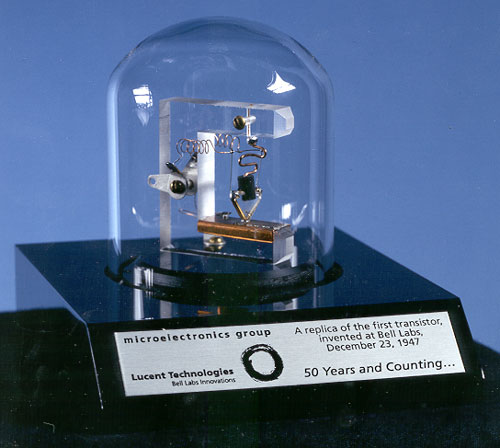
\includegraphics[width=0.45\linewidth]{images/book5/photo-first-transistor.jpg}

{\small पहले ट्रांज़िस्टर की प्रतिकृति (बेल प्रयोगशालाएँ, 1947, सार्वजनिक डोमेन): जर्मेनियम की एक फाँक पर दबे सोने के दो संपर्क। बैंड सिद्धांत की पहली मशीन --- और, वंश-परंपरा से, बाकी सारी भी।}
\end{omfigure}

\section{समस्या: छत का जनमत-संग्रह}

\begin{problem}\label{pb:b3:electrons-in-solids:1}
\emph{छत का जनमत-संग्रह।} आपका पड़ोसी तय कर रहा है कि अपने घर की छत
प्रकाश-वोल्टीय पैनलों से ढँकी जाए या नहीं, और उसने आपको, यानी
भौतिकीविद् को, मध्यस्थ नियुक्त किया है। उम्मीदवार पैनल: सिलिकॉन,
\qty{2}{m^2}, श्रेणी में साठ सेल, और दोपहर की धूप के मानक
\qty{1000}{W/m^2} के नीचे \qty{400}{W} की रेटिंग।

\medskip\noindent\textbf{भाग I --- धूप अंतराल से मिलती है।}

\begin{enumerate}
  \item सूर्य-प्रकाश मोटे तौर पर \qty{5800}{K} का तापीय वर्णक्रम है
        (\cref{ch:b3:photons-phonons}): उसके शिखर-फ़ोटॉनों की ऊर्जा
        eV में निकालिए (वीन)।
  \item सिलिकॉन का अंतराल \qty{1.12}{eV} है: कोई सिलिकॉन सेल
        अधिक से अधिक कितनी लंबी तरंगदैर्घ्य बटोर सकता है?
  \item सूर्य की मोटे तौर पर पाँचवाँ भाग शक्ति अंतराल से नीचे के
        फ़ोटॉनों में आती है। पैनल में उसका क्या होता है?
  \item कोई \qty{2.5}{eV} का हरा फ़ोटॉन अवशोषित होता है: उसकी कितनी
        ऊर्जा इलेक्ट्रॉन--विवर युग्म की ऊर्जा बनकर बचती है, और बाकी
        कहाँ जाती है, और कितनी तेज़ी से?
  \item मद 3 और 4 को वर्णक्रम के फ़ैसले में जोड़िए: कोई भी
        इलेक्ट्रॉनिकी शुरू होने से पहले ही आपाती शक्ति की लगभग आधी
        जा चुकी होती है। दोनों हानि-वाहिकाएँ एक-एक वाक्य में बताइए।
  \item किसी फ़ोटॉन को $\ge E_{\text{g}}$ की ज़रूरत ही क्यों है ---
        साधारण सिलिकॉन में झटपट एक के बाद एक आधे-अंतराल वाले दो
        फ़ोटॉन सोखने से कौन रोकता है?
\end{enumerate}

\medskip\noindent\textbf{भाग II --- इंजन के रूप में संधि।}

\begin{enumerate}[resume]
  \item हर सेल एक \omterm{prop:b3:electrons-in-solids:junction}{P--N संधि} है। तीन वाक्यों में समझाइए
        कि \omterm{prop:b3:electrons-in-solids:junction}{अवक्षय क्षेत्र} का अंतर्निर्मित क्षेत्र किसी बने हुए
        युग्म को बाहरी धारा में कैसे बदल देता है --- कौन-सा वाहक
        किस ओर जाता है, और वे बस पुनर्योजित क्यों नहीं हो जाते।
  \item $N_{\text{a}} = N_{\text{d}} = \qty{1e22}{m^{-3}}$
        और $n_{\text{i}} = \qty{1e16}{m^{-3}}$ के साथ
        \qty{300}{K} पर $V_{\text{bi}}$ निकालिए।
  \item कोई काम करता सेल लगभग \qty{0.6}{V} देता है। श्रेणी में साठ:
        पैनल की कार्यकारी वोल्टता?
  \item \qty{400}{W} की रेटिंग से कार्यकारी धारा निकालिए।
  \item प्रति अवशोषित फ़ोटॉन $\sim\qty{2}{eV}$ लेकर वह फ़ोटॉन-अभिवाह
        (प्रति सेकंड फ़ोटॉन) आकलिए जो पैनल उपयोगी ढंग से सोखता है,
        और उसकी तुलना उस इलेक्ट्रॉन-अभिवाह से कीजिए जो आपकी धारा
        कहती है: अवशोषित फ़ोटॉनों का कितना अंश कोई बटोरा गया
        इलेक्ट्रॉन देता है?
  \item निर्धारित दक्षता: \qty{2000}{W} आपाती में से
        \qty{400}{W}। भाग I के ``इलेक्ट्रॉनिकी से पहले ही आधी
        गई'' के साथ 20\,\% को मिलाइए: बाकी तीस अंक कहाँ जाते हैं?
  \item वह सेल अंतराल के पूरे \qty{1.12}{V} के बजाय
        \qty{0.6}{V} ही क्यों देता है? (डायोड के नियम में अपराधी का
        नाम लीजिए।)
\end{enumerate}

\medskip\noindent\textbf{भाग III --- असली छतें।}

\begin{enumerate}[resume]
  \item अक्षांश $50^\circ$ पर सर्दियों की किसी बादल-रहित दोपहर
        प्रकाश $30^\circ$ की ऊँचाई पर आता है। किसी क्षैतिज पैनल पर
        लंबवत आपतन के सापेक्ष ज्यामितीय गुणक
        निकालिए।
  \item पैनल का आँकड़ा-पत्रक उत्पादन का $-0.4\,\%/\text{K}$ बताता
        है: गर्मियों में कोई काली छत का पैनल \qty{65}{\celsius} तक
        पहुँच जाता है। रेटिंग का कितना बचता है?
  \item उस ताप-हानि को \cref{exo:b3:electrons-in-solids:12}(घ) से
        समझाइए।
  \item कोई चिमनी साठ में से एक सेल पर छाया डालती है। वह पूरी
        श्रेणी-लड़ी का गला क्यों घोंट सकती है --- और उस बेचारे छाया
        वाले सेल के साथ उसका अपना डायोड-स्वभाव क्या करता है?
  \item निर्माता हर उप-लड़ी के पार एक \emph{बाईपास डायोड} जोड़
        देते हैं: एक वाक्य में उसका काम समझाइए।
  \item दिनों और मौसम पर औसत लेने पर वह छत निर्धारित शक्ति का
        \qty{15}{\percent} देती है। \qty{400}{W} के पैनल से वार्षिक
        ऊर्जा किलोवाट-घंटों में आकलिए।
\end{enumerate}

\medskip\noindent\textbf{भाग IV --- फ़ैसला।}

\begin{enumerate}[resume]
  \item प्रति \unit{kWh} 0.25 यूरो पर वह पैनल साल भर में कितना
        कमाता है? और 300 यूरो की स्थापित लागत के साथ
        प्रतिदाय-काल क्या है?
  \item उस पैनल को बनाने में मोटे तौर पर \qty{500}{kWh} लगे
        (सिलिकॉन पिघलाकर शुद्ध किया जाता है): वह अपनी ही ऊर्जा
        कब तक लौटा देगा?
  \item आपका पड़ोसी पूछता है कि अंतराल से नीचे वाला पाँचवाँ भाग
        पकड़ने के लिए पैनल को ``बस काला'' क्यों नहीं बना देते।
        दो वाक्यों में बैंड सिद्धांत से उत्तर दीजिए।
  \item फिर वह पूछता है कि नीचे कोई दूसरा, छोटे अंतराल वाला पैनल
        क्यों न चढ़ा दें: \cref{exo:b3:electrons-in-solids:12}(ग)
        से उत्तर दीजिए --- और उसका व्यावहारिक
        पेच भी बताइए।
  \item तीस वर्ष बाद वह पैनल फीका पड़कर अपनी रेटिंग का 85\,\% रह
        गया है। इस अध्याय के कौन-से सूक्ष्म खलनायक
        (याद कीजिए कि $\tau$ को क्या सीमित करता है, और संधियाँ किससे
        डरती हैं) किसी सेल को बुढ़ा सकते हैं?
  \item मध्यस्थ का सार चार पंक्तियों में दीजिए: अंतराल की भौतिकी
        फ़सल तय करती है, संधि उसे बदलती है, श्रेणी-तारबंदी और ताप
        उस पर कर लगाते हैं, और बहीखाता --- ऊर्जा तथा यूरो, दोनों का
        --- पैनल के पक्ष में बंद होता है।
\end{enumerate}
\end{problem}
